\documentclass[11pt,letterpaper]{article}
\usepackage{geometry}
\geometry{margin=1in}
\usepackage{graphicx}
\usepackage{float}
\usepackage[hidelinks]{hyperref}

\setlength{\parindent}{0pt}
\setlength{\parskip}{0.5em}

%make lists tighter
\usepackage{enumitem}
\setlist{nolistsep}

%reduce spacing before and after section
\usepackage{titlesec}
\titlespacing\section{0pt}{6pt}{0pt}

\title{Lab 1 STAT 214, Spring 2026}

\author{Anonymous}

\begin{document}
\maketitle

\section{Introduction}\label{introduction}

Traumatic brain injury (TBI) is a leading cause of death and disability among children. In the emergency department, clinicians must quickly decide which pediatric head trauma patients require a CT scan. CT is highly sensitive for intracranial injury but exposes children to ionizing radiation with long-term cancer risk---particularly for young children, whose developing brains are more radiosensitive. The PECARN clinical decision rule (Kuppermann2009) addresses this trade-off by stratifying patients by age ($<$2 vs $\ge$2 years) and applying high-risk criteria (GCS$\le$14, altered mental status, skull fracture signs) and medium-risk criteria (vomiting, LOC, severe injury mechanism, severe headache, etc.) to identify children at very low risk who can safely forego imaging. Patients with no risk factors are classified as very low risk.

This report performs exploratory data analysis and preprocessing on the PECARN TBI dataset. We examine data quality, clean the data according to documented conventions, and explore \emph{interactions} between variables---how collapsing subtypes hides heterogeneity, how omitted predictors create blind spots, and how symptom effects depend on anatomical context. We then implement three classifiers (the PECARN rule, logistic regression, and random forest) and assess their diagnostic performance, interpretability, and stability. Section~2 describes data, cleaning, and exploration; Section~3 presents three findings, a reality check, and a stability check; Section~4 details modeling; Section~5 discusses limitations; Section~6 concludes. Throughout, we ground our analyses in the clinical context of pediatric head trauma decision-making.

\section{Data}\label{data}

The dataset consists of 43,399 pediatric patients (under 18 years) evaluated for head trauma at 25 PECARN emergency departments. It contains 125 variables covering demographics, injury mechanism, signs and symptoms (loss of consciousness, vomiting, headache), Glasgow Coma Scale (GCS) components, and outcomes including CT results and clinically important TBI (ciTBI).

\subsection{Data Collection}\label{data-collection}

Trained site investigators recorded patient history, injury mechanism, and clinical signs on standardized forms \emph{before} imaging results were known. Data were collected prospectively from patients presenting within 24 hours of head trauma. This design reduces recall bias and ensures predictor--outcome independence. The multi-site design (25 EDs) improves generalizability but introduces potential site-level variation in patient populations and data entry practices. The study excluded children with trivial injury mechanisms (ground-level falls with no signs beyond scalp abrasions); our cohort therefore represents a population with at least some clinical concern, which may explain the non-negligible PosCT rate (5--6\%) among imaged patients.

Variables span binary indicators (vomiting yes/no), ordinal categories (injury severity: low/moderate/high), and numeric values (age in months, GCS). Many have conditional structure: LocLen is recorded only when LOC is present, HASeverity only when headache is present. This creates structured missingness where ``not applicable'' must be distinguished from truly missing data. The documentation encodes these distinctions (code 92 for ``not applicable''), which we leverage during cleaning.

\subsection{Data Cleaning}\label{data-cleaning}

\textbf{Missing value codes.} The documentation specifies that missingness is encoded numerically: 91 (pre-verbal/non-verbal), 92 (not applicable), 99 (unknown/refused), 90 (other), and $-1$. We replace all such codes with NaN across 81 columns for consistent handling. Treating 92 as ``not applicable'' is conceptually distinct from ``unknown'' (99), but for most analyses we treat both as missing for simplicity and consistency. For PosCT and EDCT, code 92 (no CT performed) means no outcome is available, so we exclude such rows from the modeling cohort.

\textbf{Consistency checks.} In 56 rows, the sum of GCS components (eye 1--4, verbal 1--5, motor 1--6) does not equal the recorded GCSTotal, suggesting data entry error. We flag but retain these rows, as the recorded total may still be clinically valid. We verified that AgeTwoPlus is fully consistent with AgeInMonth: every patient's age-group assignment matches the value derived from AgeInMonth (AgeTwoPlus$=$1 when AgeInMonth $<$ 24; AgeTwoPlus$=$2 when $\ge$ 24).

\textbf{Outcome variables.} PosCT is missing when CT was not performed; we restrict modeling to the subset with CT done and non-missing PosCT ($n=14{,}983$). We derive ciTBI as the composite of DeathTBI, Neurosurgery, Intub24Head, or PosIntFinal, following the Kuppermann definition. The broader analysis cohort (GCS 14--15, CT or outcome available) yields 42,429 patients. All preprocessing is in \texttt{clean.py}. Figure~\ref{fig:eda} shows missingness and key distributions; Figure~\ref{fig:gcs} illustrates the GCS consistency check and PECARN variable correlations.

\begin{figure}[H]
\centering
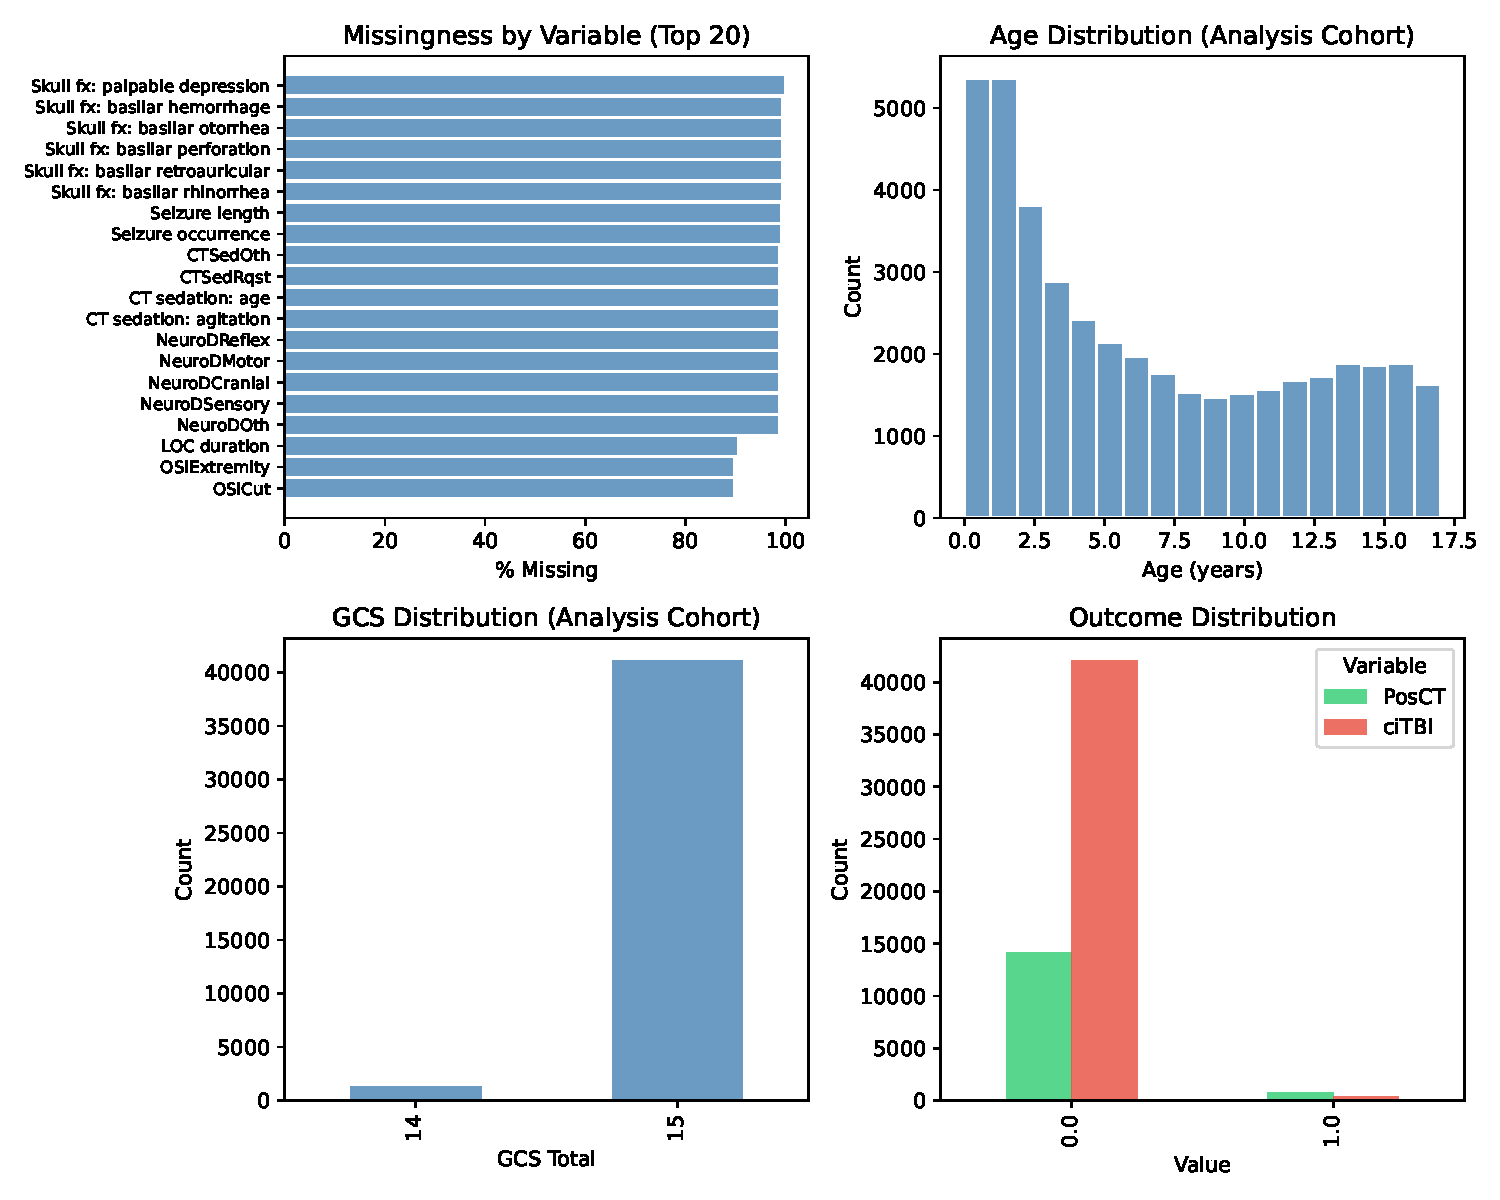
\includegraphics[width=0.82\textwidth]{figures/eda_overview.pdf}
\caption{Exploratory data overview: missingness by variable (top 20), age distribution, GCS distribution, and outcome rates in the analysis cohort.}
\label{fig:eda}
\end{figure}

\begin{figure}[H]
\centering
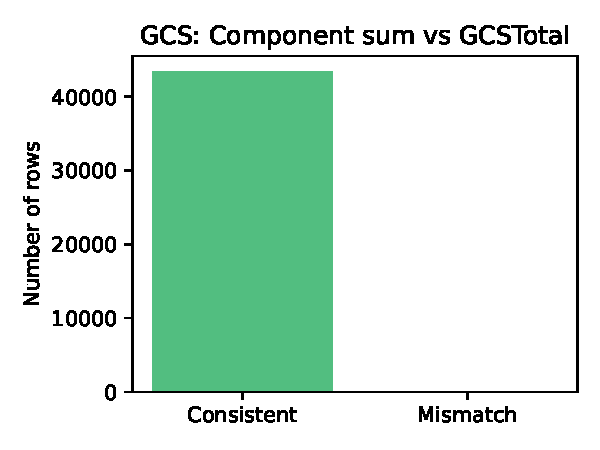
\includegraphics[width=0.3\textwidth]{figures/gcs_consistency.pdf}
\hfill
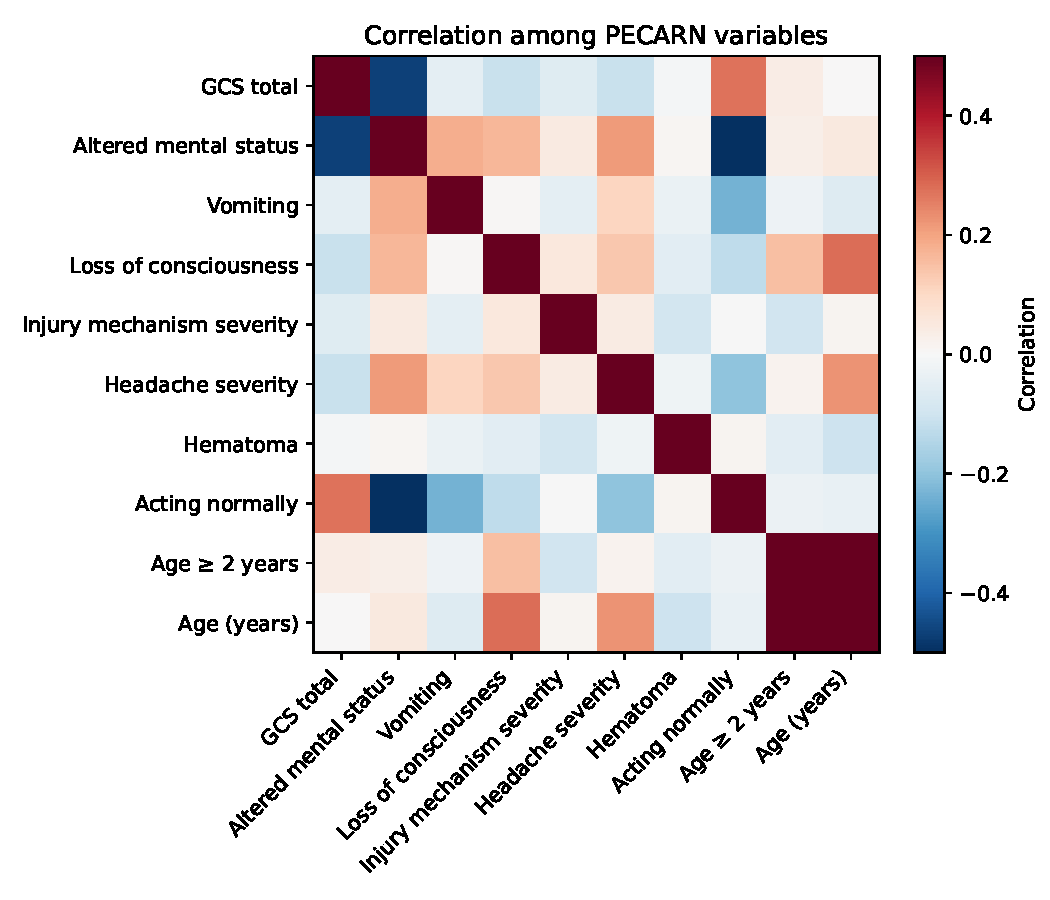
\includegraphics[width=0.5\textwidth]{figures/pecarn_correlation.pdf}
\caption{Left: GCS component sum vs GCSTotal (56 mismatches flagged). Right: Correlation heatmap among PECARN variables---symptom-based and mechanism-based clusters emerge.}
\label{fig:gcs}
\end{figure}

\subsection{Data Exploration}\label{data-exploration}

We restrict to the GCS 14--15 cohort with CT or outcome available ($n=42{,}429$). The ciTBI rate is 0.89\%, consistent with a low-risk population. Among imaged patients, the PosCT rate is 5--6\%, higher than ciTBI because PosCT captures any intracranial finding while ciTBI requires clinically important sequelae. Core variables (GCSTotal, AgeTwoPlus, Vomit, AMS) have $<$1\% missing; conditional variables (LocLen, HASeverity, HemaLoc) have high ``not applicable'' rates.

\textbf{Correlation structure.} The PECARN risk factors are not independent (Figure~\ref{fig:gcs}, right). For instance, AMS and GCS are negatively correlated, as well as acting normally and AMS. Two clusters emerge: (1) symptom-based indicators (AMS, Vomit, LOC) that co-occur; (2) mechanism/demographic variables weakly correlated with symptoms but associated with outcomes. Logistic regression may show suppressed coefficients for correlated predictors, while random forests are robust to collinearity.

\textbf{Age modifies predictor--outcome relationships.} The PECARN rule stratifies by age for good reason: predictor--outcome relationships differ substantially by age group (Figure~\ref{fig:age_strat}). Children under 2 have uniformly higher PosCT rates across all injury severity levels ($<$2: Low 3.4\%, Moderate 7.0\%, High 12.6\%; $\ge$2: Low 2.2\%, Moderate 3.7\%, High 7.9\%). The age gap is largest at moderate severity (7.0\% vs 3.7\%). AMS shows a similar age-dependent pattern. These effects validate the PECARN rule's age-stratified design.

\begin{figure}[H]
\centering
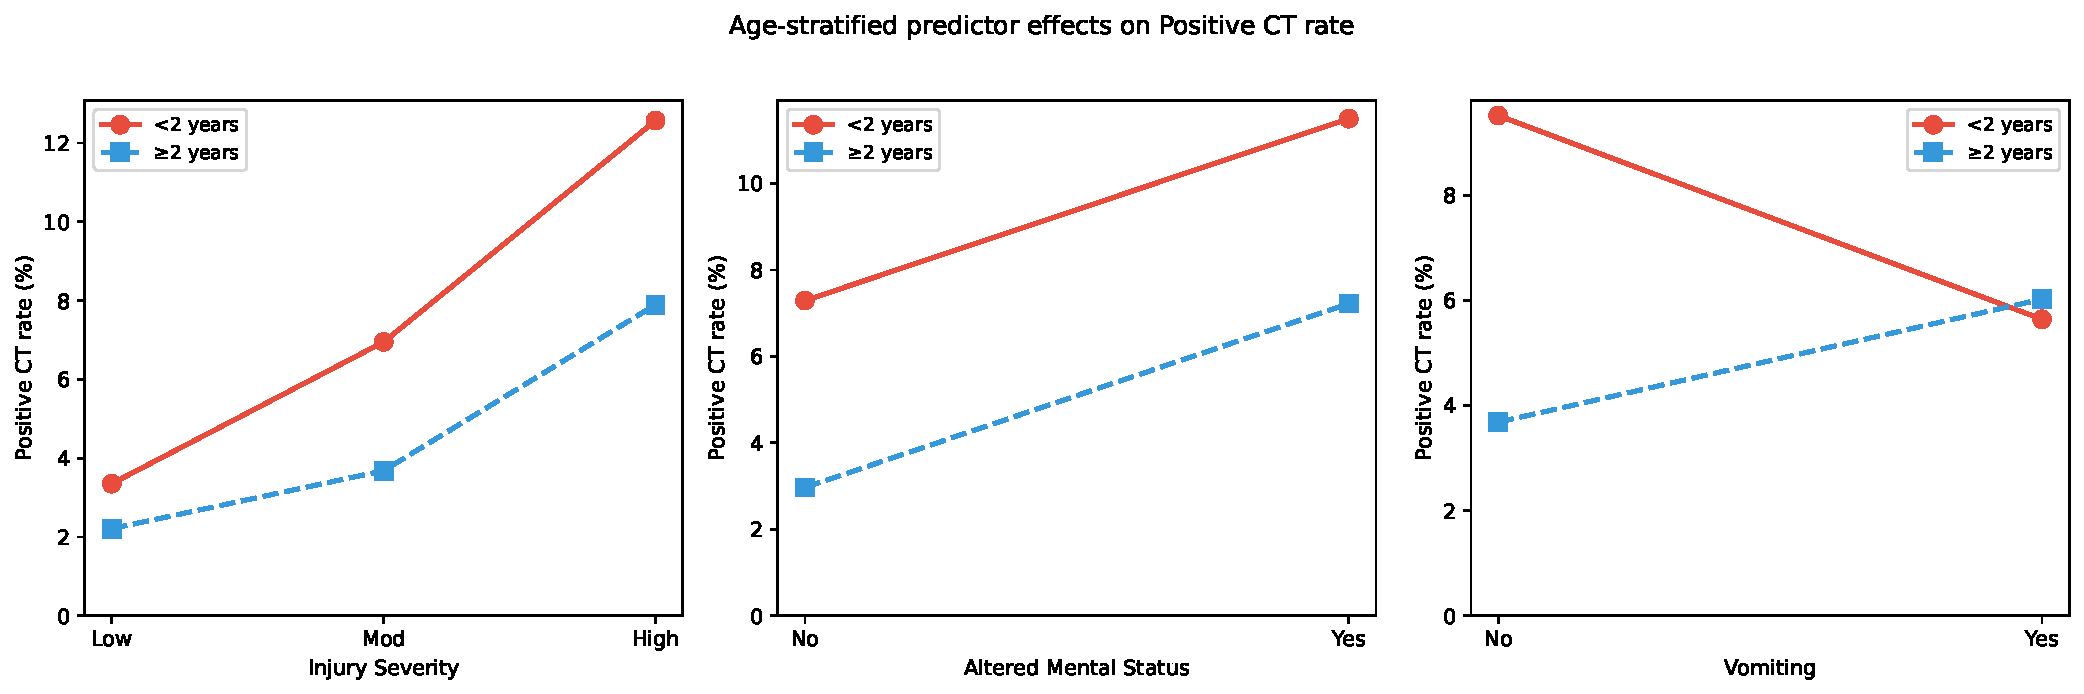
\includegraphics[width=0.82\textwidth]{figures/age_stratified_effects.pdf}
\caption{Age-stratified predictor effects. Children $<$2 years have higher PosCT rates across all levels, supporting age-stratified clinical rules.}
\label{fig:age_strat}
\end{figure}

\textbf{Selection bias in CT ordering.} Because CT is not performed on all patients, our modeling cohort is a non-random subset. CT patients have substantially higher rates of AMS (32\% vs 5\%), vomiting (25\% vs 7\%), and high-impact injury (26\% vs 15\%) compared to non-imaged patients (Figure~\ref{fig:selection_bias}). This verification bias inflates the PosCT rate in the imaging cohort and limits model generalizability to unselected populations.

\begin{figure}[H]
\centering
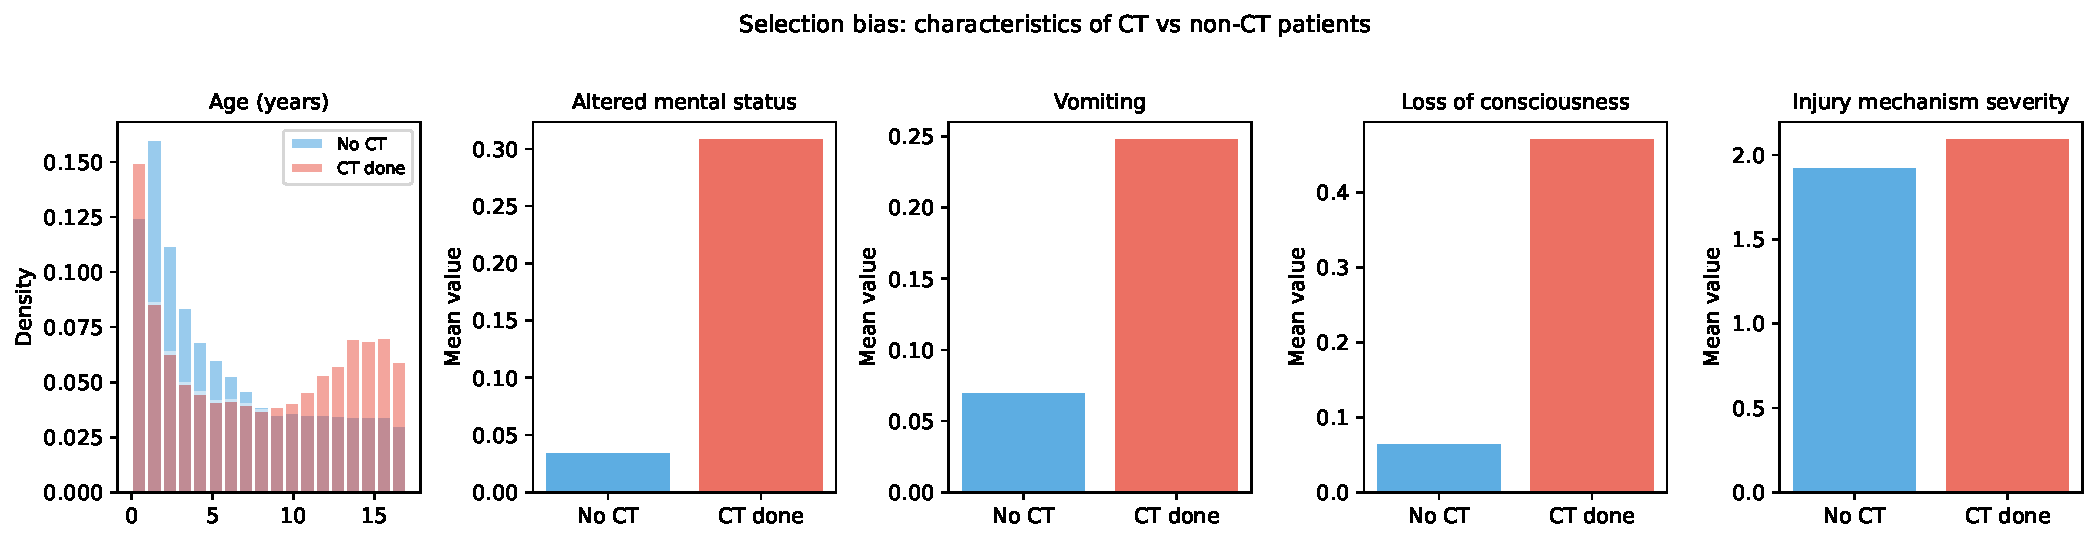
\includegraphics[width=0.95\textwidth]{figures/selection_bias.pdf}
\caption{Selection bias: CT patients have higher risk factor prevalence than non-imaged patients.}
\label{fig:selection_bias}
\end{figure}

\textbf{GCS 14 vs 15: a clinically meaningful boundary.} Within our GCS 14--15 cohort, GCS$=$14 carries a 13.7\% PosCT rate ($n=1{,}203$) versus 4.5\% for GCS$=$15 ($n=13{,}780$)---a three-fold difference (Figure~\ref{fig:gcs14v15}). GCS 14 patients also have dramatically higher prevalence of AMS, LOC, and high-impact injury mechanisms. The PECARN rule's GCS$\le$14 criterion correctly identifies these patients; our data validate this threshold. However, GCS 15 patients constitute 92\% of the cohort, so the other PECARN factors (AMS, injury severity, vomiting) drive the vast majority of clinical decisions. All three findings---AMS subtype heterogeneity (Finding 1), the seizure blind spot (Finding 2), and location-dependent vomiting (Finding 3)---are most relevant for this large GCS 15 subgroup, where the rule relies on these secondary factors to stratify risk.

\begin{figure}[H]
\centering
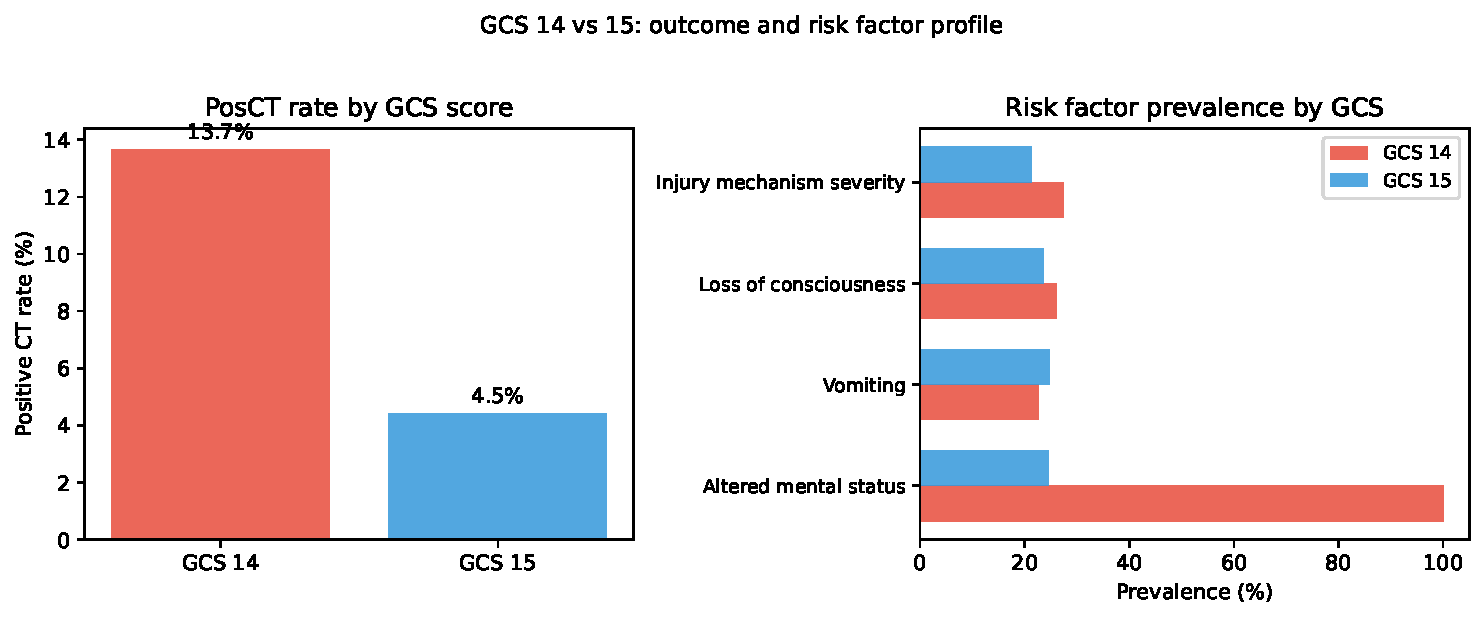
\includegraphics[width=0.7\textwidth]{figures/gcs14_vs_15.pdf}
\caption{GCS 14 vs 15: PosCT rate (left) and risk factor prevalence (right).}
\label{fig:gcs14v15}
\end{figure}

\section{Findings}\label{findings}

\subsection{First finding: AMS subtypes are not created equal---``Agitated'' signals double the risk of ``Sleepy''}\label{first-finding}

The PECARN rule treats altered mental status (AMS) as a single binary variable. However, AMS encompasses qualitatively different presentations: agitation, sleepiness, slow responsiveness, and repetitive questioning. Decomposing AMS into its subtypes reveals dramatic heterogeneity (Figure~\ref{fig:ams_subtypes}, left). Agitated children have a 15.4\% PosCT rate ($n=638$)---more than double the rate for sleepy children (7.6\%, $n=2{,}334$) and triple the rate for slow-to-respond children (6.5\%, $n=1{,}268$). Children who repeat questions fall between (9.7\%, $n=421$). All AMS subtypes exceed the no-AMS baseline (4.8\%), but the range---from 6.5\% to 15.4\%---means the binary AMS variable collapses a 2.4-fold internal gradient.

This is counter-intuitive: one might expect ``sleepy'' to signal intracranial pressure and carry the highest risk, while ``agitated'' might reflect pain or fear. Instead, agitation appears to be a stronger marker of intracranial pathology. The interaction with injury mechanism severity amplifies this (Figure~\ref{fig:ams_subtypes}, right): agitated children after a high-impact mechanism have a 23.3\% PosCT rate---nearly 1 in 4---compared to 14.7\% for sleepy children in the same scenario. The PECARN rule's binary treatment of AMS obscures this clinically actionable heterogeneity. Under cohort perturbation (excluding age $<$2), the pattern persists: agitated remains the highest-risk subtype at 16.2\%.

\begin{figure}[H]
\centering
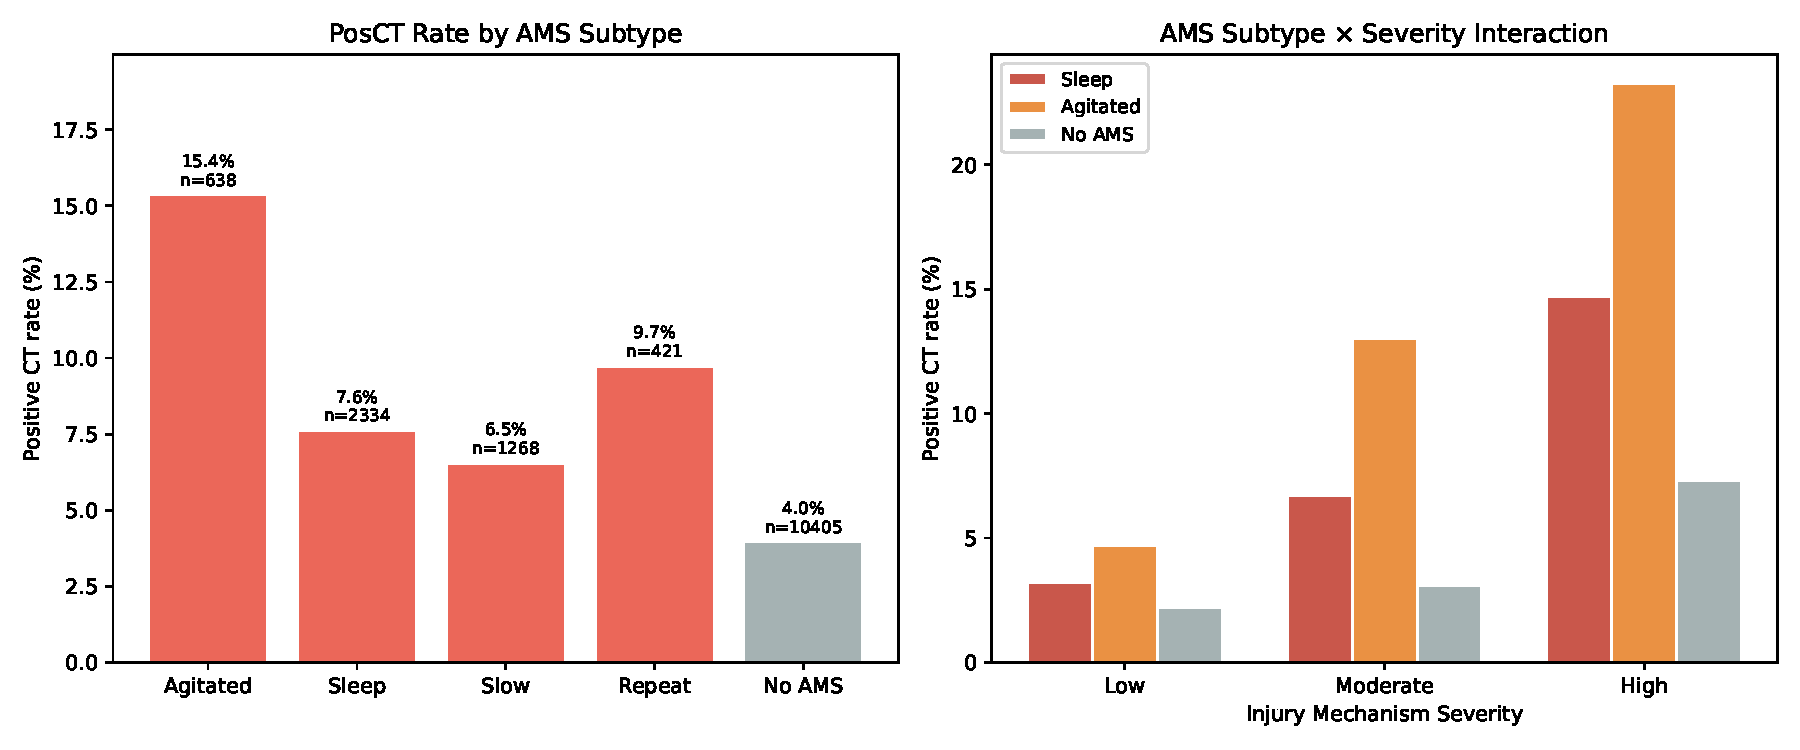
\includegraphics[width=0.9\textwidth]{figures/finding_ams_subtypes.pdf}
\caption{Left: PosCT rate by AMS subtype---``Agitated'' (15.4\%) is more than double ``Sleepy'' (7.6\%). Right: AMS subtype $\times$ injury severity interaction. Agitated + high-impact reaches 23.3\%.}
\label{fig:ams_subtypes}
\end{figure}

\subsection{Second finding: Post-traumatic seizures are a PECARN blind spot}\label{second-finding}

Post-traumatic seizures are explicitly absent from the PECARN decision rule, yet patients with seizures have a 7.0\% PosCT rate ($n=412$)---higher than vomiting (5.9\%), loss of consciousness (5.1\%), and comparable to AMS (8.1\%), all of which are PECARN risk factors (Figure~\ref{fig:seizures}, right). The omission means the rule does not flag seizure patients for imaging unless they also exhibit a listed risk factor.

The seizure effect is most pronounced in older children: among patients $\ge$2 years, seizure raises the PosCT rate from 4.2\% to 6.5\%---a 55\% relative increase (Figure~\ref{fig:seizures}, left). In the $<$2 group, rates are similar with and without seizure (8.9\% vs 8.5\%), likely because the high baseline risk in infants masks the seizure signal. Critically, among patients with zero PECARN risk factors---those the rule classifies as ``very low risk''---seizure doubles the PosCT rate from 1.6\% to 3.4\%. Although this subgroup is small ($n=58$), the pattern suggests the rule has a blind spot: patients who seize but have no other PECARN flags may still warrant imaging. Under perturbation, the seizure effect persists (6.5\% vs 4.2\% in the $\ge$2 cohort).

\begin{figure}[H]
\centering
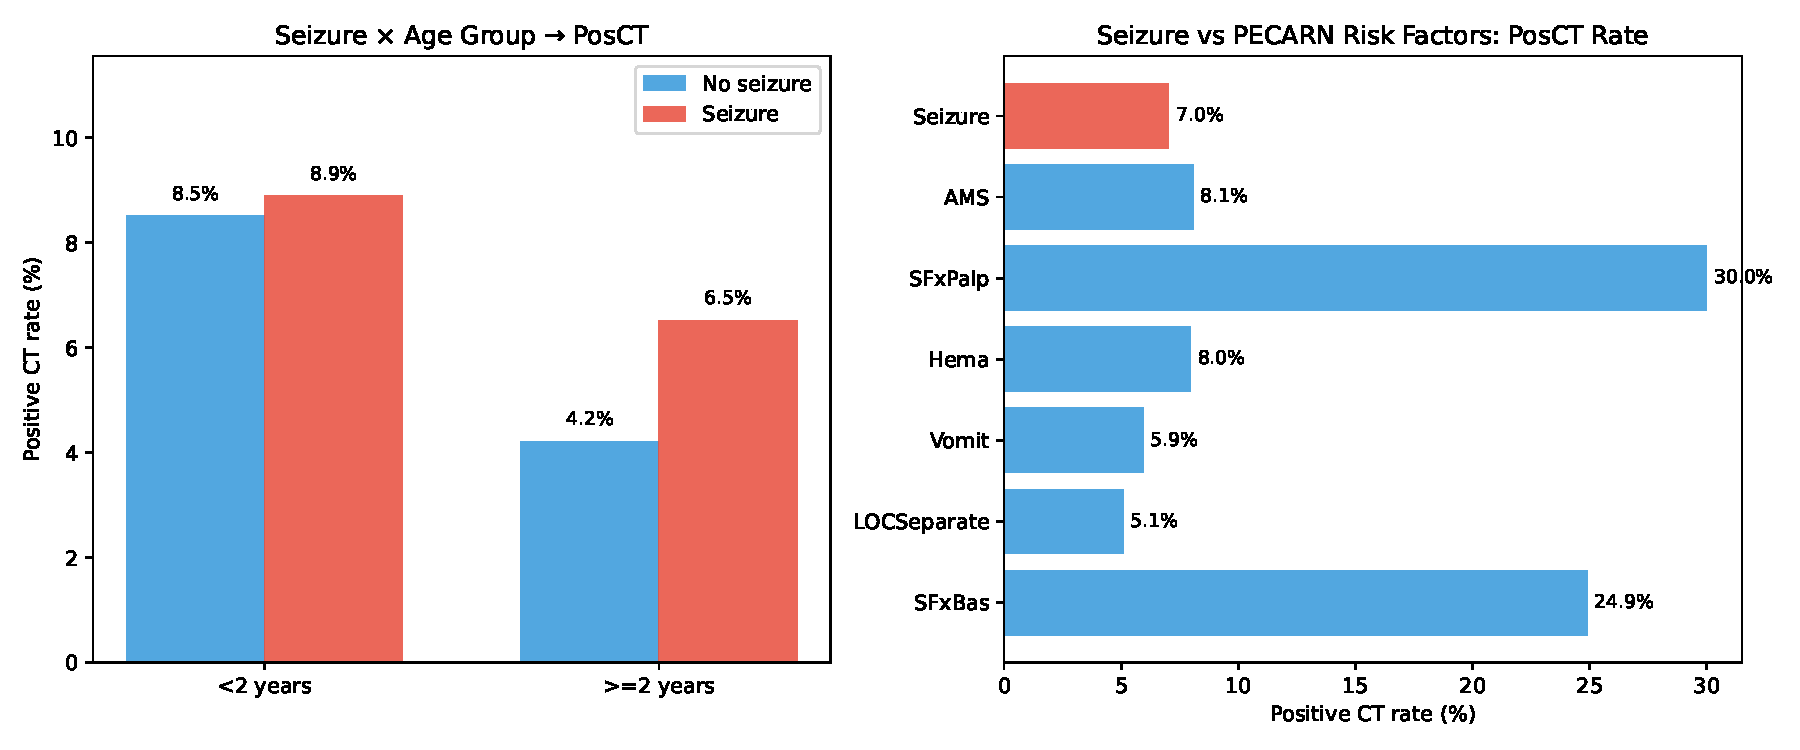
\includegraphics[width=0.9\textwidth]{figures/finding_seizures.pdf}
\caption{Left: Seizure $\times$ age group. Seizures raise PosCT by 55\% in $\ge$2 years. Right: Seizure PosCT (7.0\%) compared to each PECARN risk factor---it ranks alongside AMS and above vomiting and LOC.}
\label{fig:seizures}
\end{figure}

\subsection{Third finding: Vomiting is a location-dependent risk amplifier---occipital hematoma with vomiting and LOC reaches 21\%}\label{third-finding}

The PECARN rule uses hematoma location only for children $<$2 years (non-frontal hematoma is a medium-risk criterion) and treats vomiting and LOC as location-independent binary triggers. Our analysis reveals that vomiting's predictive power depends entirely on hematoma location (Figure~\ref{fig:hemaloc_compound}, left). At the frontal location, vomiting has \emph{no effect}: 4.0\% without vomiting vs 3.7\% with. But at temporal/parietal locations, vomiting raises risk by 75\% (6.3\% $\to$ 11.0\%), and at occipital locations by 27\% (12.6\% $\to$ 16.0\%). The PECARN rule's uniform treatment of vomiting misses this location-dependent amplification.

The compound effect is most striking when vomiting and LOC co-occur at non-frontal locations: occipital hematoma with both vomiting and LOC yields a 21.3\% PosCT rate ($n=108$)---more than 1 in 5. Temporal/parietal with both symptoms reaches 18.1\% ($n=72$). By contrast, frontal hematoma with both symptoms is only 9.8\%---half the occipital rate. This three-way interaction (location $\times$ vomiting $\times$ LOC) identifies a high-risk subgroup that the PECARN rule does not distinguish from patients with a single symptom at any location.

Gender, though nearly irrelevant overall (male 5.3\%, female 5.2\%), introduces a further asymmetry (Figure~\ref{fig:hemaloc_compound}, right): males with occipital hematoma and vomiting have a 16.7\% rate versus 14.8\% for females; but females with frontal hematoma and LOC have an 8.7\% rate versus 4.9\% for males. Under perturbation (excluding $<$2 years), the location $\times$ vomiting interaction persists (occipital+vomit: 15.1\%, temp/parietal+vomit: 11.8\%, frontal+vomit: 3.6\%).

\begin{figure}[H]
\centering
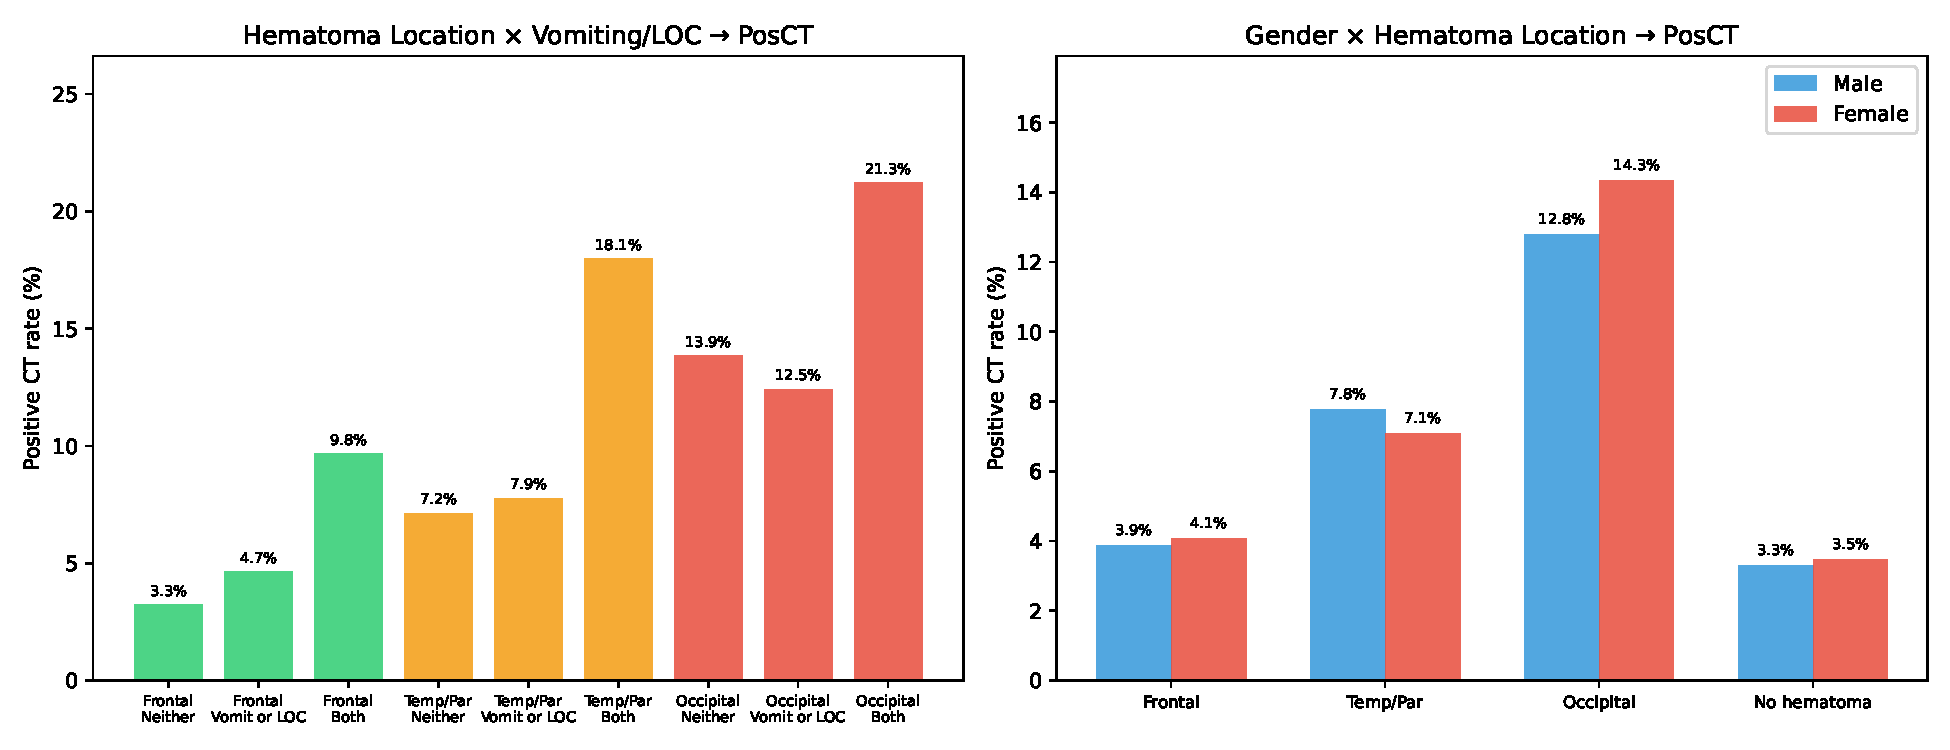
\includegraphics[width=0.95\textwidth]{figures/finding_hemaloc_compound.pdf}
\caption{Left: Hematoma location $\times$ vomiting/LOC. Vomiting amplifies risk at non-frontal locations but has no effect at frontal. Occipital + both symptoms = 21.3\%. Right: Gender $\times$ location---males show slightly higher occipital risk, females show elevated frontal+LOC risk.}
\label{fig:hemaloc_compound}
\end{figure}

\subsection{Reality Check}\label{reality-check}

We compare our cleaned data to external benchmarks. \textbf{Assumptions:} (1) The published PECARN population is comparable to our cohort; (2) ciTBI is rare in GCS 14--15 patients; (3) the PosCT rate should fall in 3--10\% for mild head trauma.

\textbf{Findings:} Our ciTBI rate (0.89\%) aligns with Kuppermann et al.'s ``very low risk'' framing. Kuppermann et al.\ reported sensitivity of 100\% (for $<$2 years) and 96.8\% (for $\ge$2 years) for ciTBI, implying ciTBI is rare in the population the rule screens. The PosCT rate among imaged patients (5--6\%) falls within the expected 3--10\% range for mild head trauma. The age distribution (median $\sim$6 years) and injury mechanism distribution match typical pediatric ED populations. The GCS mismatch (56 rows) is a documented limitation; AgeTwoPlus is fully consistent with AgeInMonth. Our cleaning did not introduce obvious distortion; a stronger check would use independent validation data.

\subsection{Stability Check}\label{stability-check}

We perturbed the cohort by excluding children under 2 ($\sim$22\% of patients). All three findings are robust. Finding 1: AMSAgitated remains the highest-risk subtype (16.2\% in the perturbed cohort vs 15.4\% in the full cohort); the subtype ordering is preserved. Finding 2: the seizure effect persists---6.5\% vs 4.2\% among $\ge$2 years. Finding 3: the location-dependent vomiting interaction persists (occipital+vomit: 15.1\%, temporal/parietal+vomit: 11.8\%, frontal+vomit: 3.6\%)---the amplification pattern is stable and not driven by the infant subgroup. Figure~\ref{fig:stability} illustrates the injury-severity gradient before and after perturbation as an additional baseline check.

\begin{figure}[H]
\centering
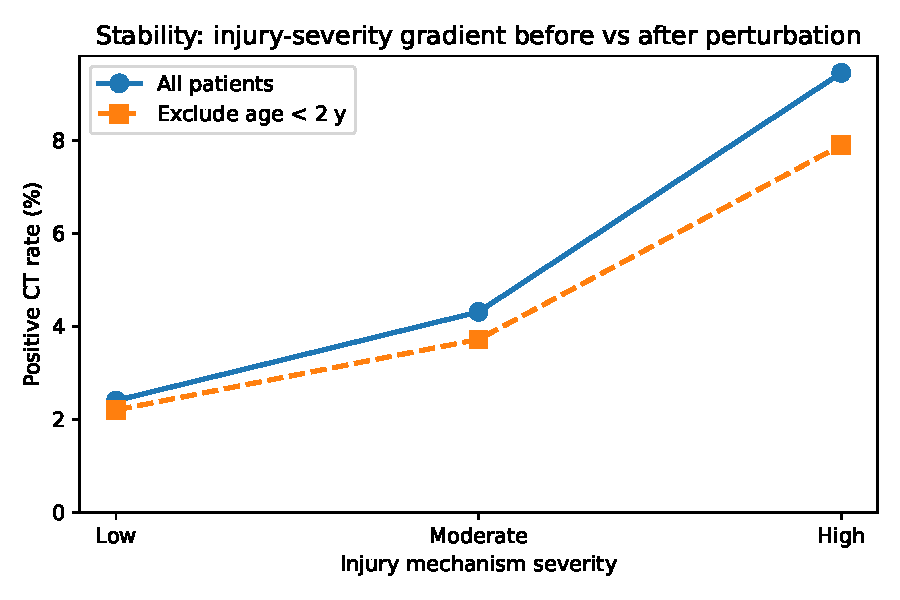
\includegraphics[width=0.55\textwidth]{figures/stability_check.pdf}
\caption{Stability check: injury severity gradient before and after excluding age $<$2 years. The monotonic dose-response is preserved under perturbation.}
\label{fig:stability}
\end{figure}

\section{Modeling}

\subsection{Implementation}

We implemented three classifiers to predict PosCT among imaged patients. (1)~\textbf{PECARN rule:} Applied as specified by Kuppermann et al.\ for age $<$2 and $\ge$2, outputting a binary CT recommendation. (2)~\textbf{Logistic regression:} L2-regularized (C=1) on all 17 PECARN risk factors from Kuppermann et al.: GCSTotal, AMS, High\_impact\_InjSev, SFxPalp, Hema, HemaLoc, LocLen, ActNorm (for $<$2 years), SFxBas and subtypes, Vomit, LOCSeparate, HASeverity (for $\ge$2 years), with standardization. Age is excluded because the PECARN rule uses it as a stratification variable, not a risk factor. Missing values imputed with 0 (e.g., LocLen$=$0 interpreted as ``no LOC''). (3)~\textbf{Random forest:} 100 trees, max depth 10, same feature set. We used a 75--25 train-test split (random\_state=42). We chose C=1 (moderate regularization) and max\_depth=10 as reasonable defaults; formal hyperparameter tuning via cross-validation could be explored in future work. Additionally, to address class imbalance, we re-fit both ML models with \texttt{class\_weight="balanced"}, inversely weighting each class by frequency ($\sim$18$\times$ weight for the minority class).

Figure~\ref{fig:model_comp} compares accuracy. The PECARN rule achieves $\sim$26\% accuracy---not because it is poorly designed, but because it optimizes sensitivity over specificity. The rule recommends CT for most patients to avoid missed diagnoses; when 94\% of patients have negative CT, a rule that recommends CT for most will correctly predict ``positive'' for only a small fraction. Logistic regression and random forest achieve $\sim$95\% accuracy by predicting negative CT for most patients, matching the class distribution. However, high accuracy in an imbalanced setting is misleading: a naive ``always predict negative'' rule achieves 94\%. The relevant comparison for clinical use is sensitivity (among true PosCT, how many did we flag?) and specificity (among true negatives, how many unnecessary CTs did we avoid?).

\begin{figure}[H]
\centering
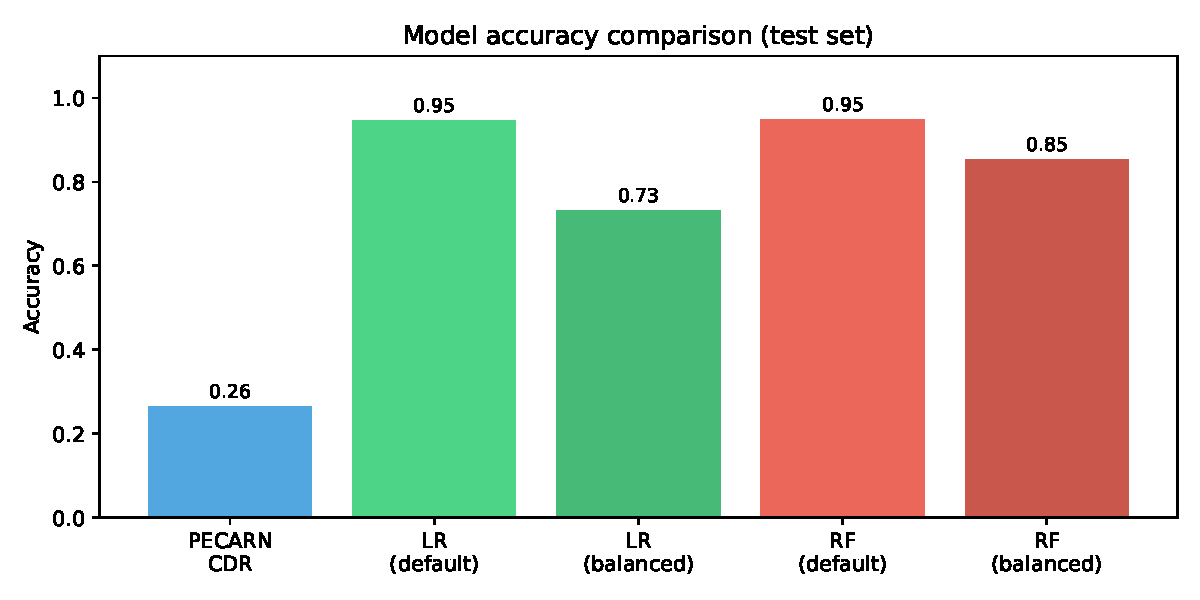
\includegraphics[width=0.45\textwidth]{figures/model_comparison.pdf}
\caption{Model accuracy on the test set. PECARN prioritizes sensitivity over accuracy.}
\label{fig:model_comp}
\end{figure}

\subsection{Diagnostic Performance}

Figure~\ref{fig:diag_perf} reveals the core trade-off. The PECARN rule achieves 92.4\% sensitivity but only 22.8\% specificity (PPV$=$6.2\%, NPV$=$98.2\%): it flags nearly all positive cases at the cost of many unnecessary CTs. The default-threshold ML models show the opposite: $>$99.6\% specificity but only 5--7\% sensitivity, because the 0.5 decision threshold is far above the 5.3\% base rate.

\begin{figure}[H]
\centering
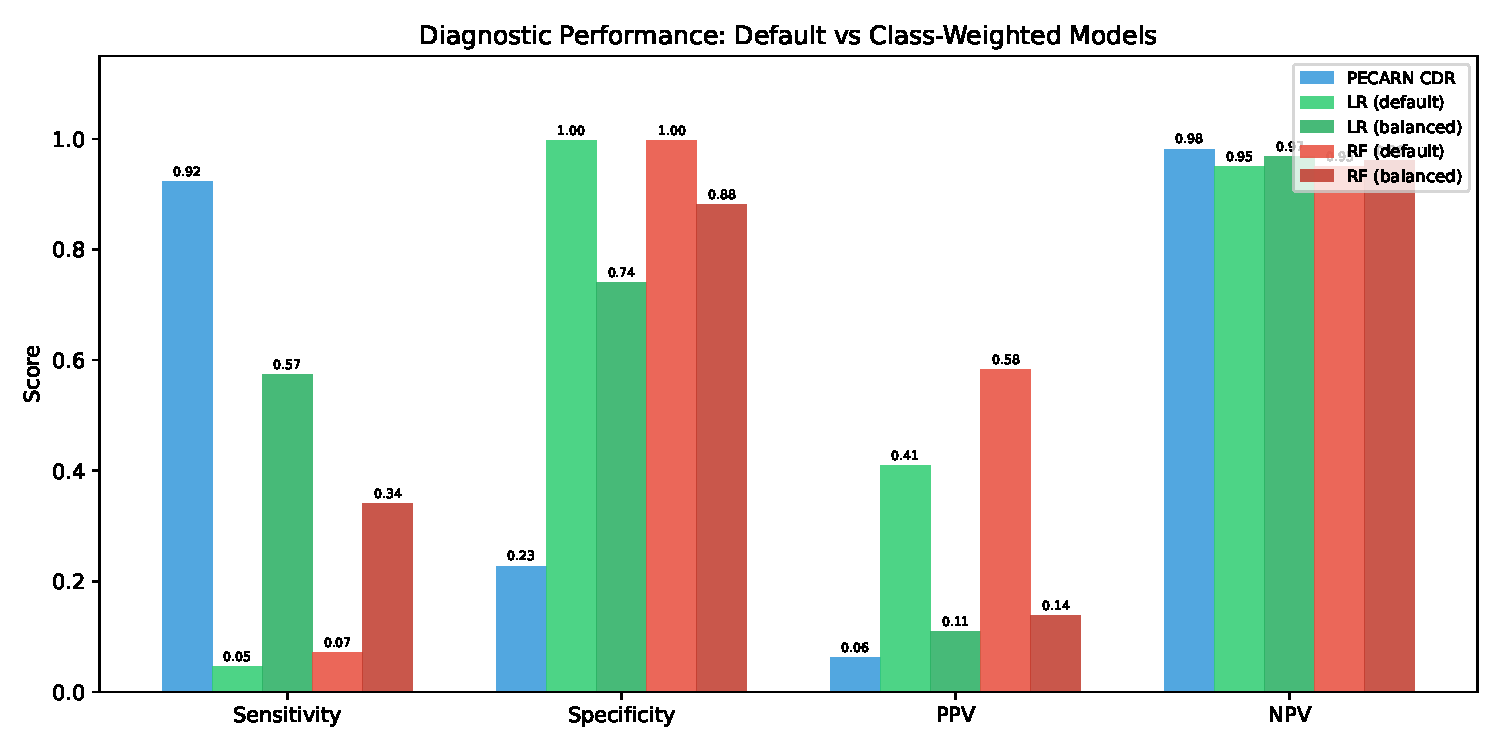
\includegraphics[width=0.85\textwidth]{figures/diagnostic_performance.pdf}
\caption{Diagnostic performance: default and class-weighted models. PECARN achieves high sensitivity; class-weighted models partially close the gap but do not match it.}
\label{fig:diag_perf}
\end{figure}

\textbf{Class-weighted models.} With balanced class weights, the logistic regression achieves 57.4\% sensitivity and 74.1\% specificity (PPV$=$10.9\%, NPV$=$96.9\%); the random forest achieves 34.0\% sensitivity and 88.2\% specificity (PPV$=$13.8\%, NPV$=$96.0\%). The class-weighted LR substantially improves over the default---sensitivity rises from 5\% to 57.4\%---but remains far below PECARN's 92.4\%. The class-weighted RF is more conservative, trading sensitivity for higher specificity. Figure~\ref{fig:threshold_comparison} places all variants in the sensitivity--specificity plane: PECARN occupies the upper-left; default ML models sit in the lower-right; class-weighted models fall between. No ML variant dominates PECARN in both dimensions, confirming that cost-sensitive training alone cannot replicate the rule's expert-designed, age-stratified logic.

\begin{figure}[H]
\centering
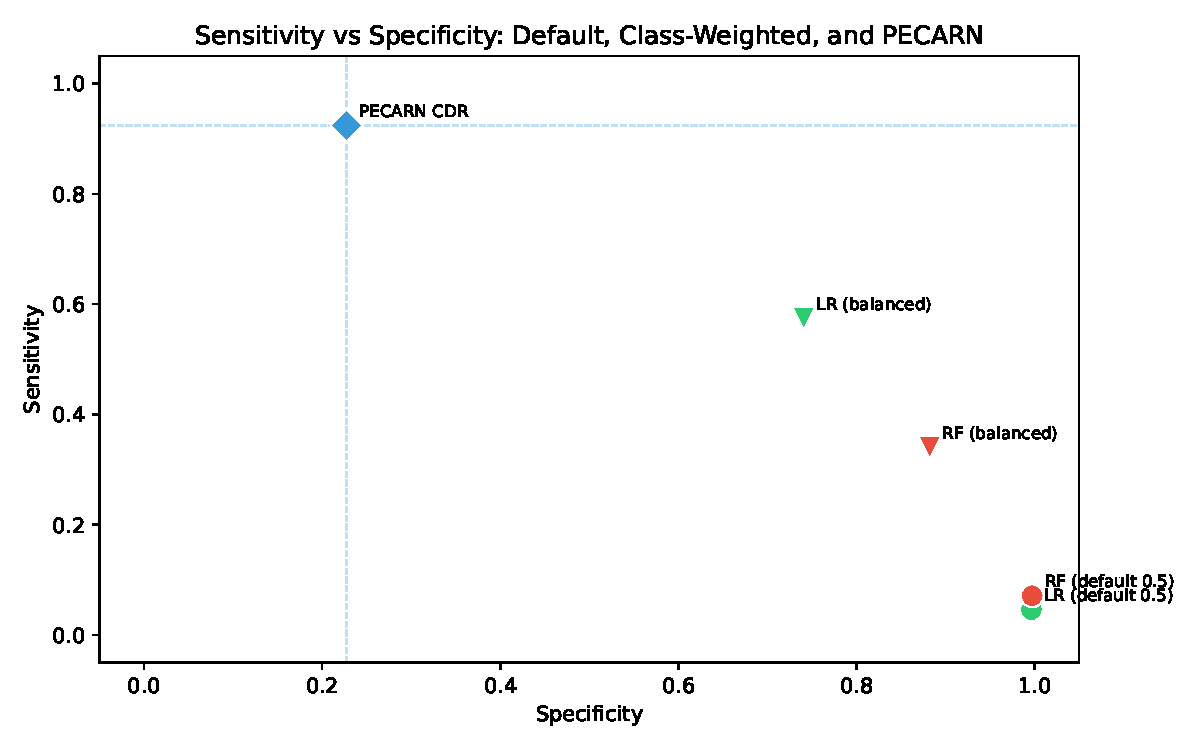
\includegraphics[width=0.7\textwidth]{figures/threshold_comparison.pdf}
\caption{Sensitivity vs.\ specificity across model variants. No ML variant dominates the PECARN rule in both dimensions simultaneously.}
\label{fig:threshold_comparison}
\end{figure}

\subsection{Interpretability}

The PECARN rule is a bedside checklist---transparent and auditable. Logistic regression offers coefficient-based interpretability: HemaLoc has the largest positive coefficient (0.66, OR$=$1.94), followed by High\_impact\_InjSev (0.39, OR$=$1.48), AMS (0.25, OR$=$1.28), SFxPalp (0.23, OR$=$1.26), and Vomit (0.23, OR$=$1.26)---all consistent with PECARN's emphasis. GCSTotal is negative ($-$0.22, OR$=$0.80), as expected. Hema shows a negative coefficient ($-$0.20) due to collinearity with HemaLoc. Basilar skull fracture subtypes have small coefficients due to low prevalence ($<$2\%). Figure~\ref{fig:lr_coef} shows both models emphasize the same predictors---injury severity, HemaLoc, AMS in the upper-right---providing reassurance that the rule captures the right variables. Notably, HemaLoc's dominance as the strongest predictor aligns with Finding~3: hematoma location carries substantial independent signal that the rule currently uses only for $<$2 years, and its interaction with vomiting and LOC (Section~\ref{third-finding}) suggests the model is implicitly learning location-dependent risk that the rule's uniform symptom weights miss.

\begin{figure}[H]
\centering
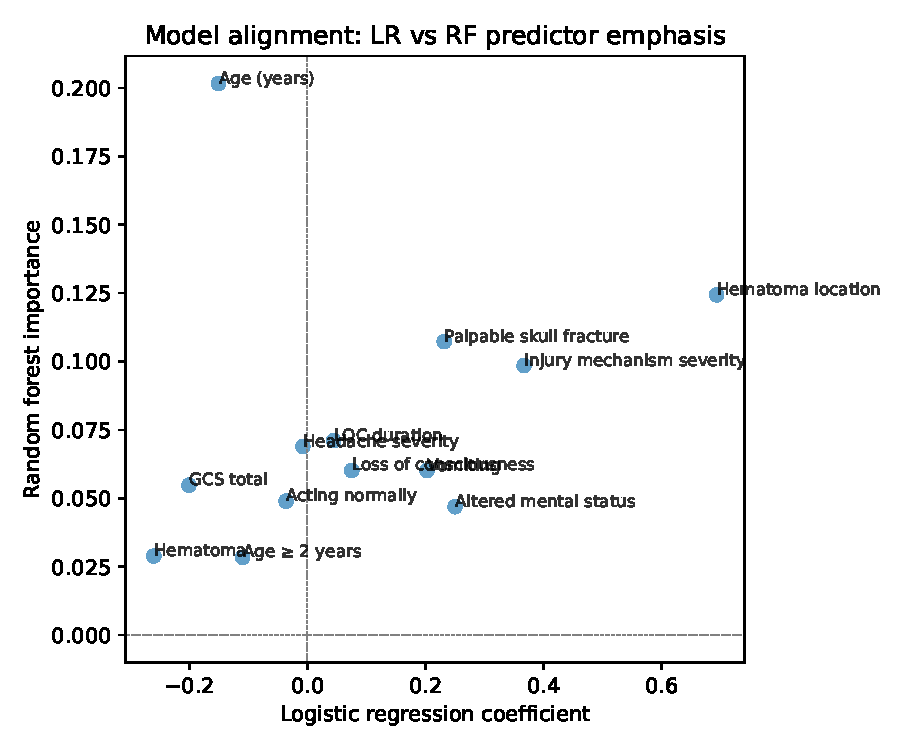
\includegraphics[width=0.55\textwidth]{figures/model_alignment.pdf}
\caption{Model alignment: LR coefficient vs RF importance. Both converge on injury severity, AMS, and hematoma location.}
\label{fig:lr_coef}
\end{figure}

\subsection{Model Stability}

Under the perturbation (excluding children under 2), the PECARN rule's $\ge$2 stratum logic is unchanged, so its behavior is stable. The ML models would change if retrained, but we expect the qualitative ranking of important predictors to persist. A full model-level stability analysis (retraining and comparing before/after) is a natural next step.

\section{Discussion}\label{discussion}

\textbf{Data size and class imbalance.} With 43,399 patients and 15,899 CT scans, the dataset supports stable marginal estimates. The main constraint is class imbalance (5--6\% PosCT, 0.89\% ciTBI), which makes accuracy misleading and motivated our class-weighted analysis. At the interaction level, subgroup sizes vary: the AMS-subtype and seizure findings rest on hundreds to thousands of patients per cell, but the three-way interaction in Finding~3 (occipital+vomit+LOC, $n=108$; temporal/parietal+vomit+LOC, $n=72$) is adequately powered for rate estimation yet too small for formal hypothesis testing.

\textbf{Data, models, and reality.} Our cleaned data approximates clinical reality imperfectly. The GCS mismatch (56 rows) reminds us that data are a filtered, digitized representation of clinical events; they are not reality itself. The PECARN rule, LR, and RF produce predictions whose validity depends on data quality; the convergence of ML predictors with the rule suggests meaningful signal, but model validity also requires that future data resemble the training population. There is no one-to-one correspondence between data and reality---visualization further compresses this representation. Transparency about preprocessing, consistency checks, and limitations is essential. Deployment on new patients requires that future data resemble the study population; generalizability to different settings (e.g., resource-limited environments, different age distributions) would require additional validation studies.

\textbf{Verification bias and selection effects.} Our modeling cohort is limited to patients who received CT---a non-random, higher-risk subset (Figure~\ref{fig:selection_bias}). This introduces \emph{verification bias}: we only observe PosCT for patients selected for imaging, and this selection correlates with the very predictors we model. Our performance metrics apply to the imaged population, not the full ED population. The PECARN rule's sensitivity (92.4\%) is measured only among those imaged; if un-imaged patients had undetected positive CT, the true sensitivity would be lower. The study's telephone follow-up for non-imaged patients mitigates this concern, but the distinction between ``predicting among imaged patients'' and ``deciding who to image'' remains important.

\textbf{Limitations.} We used simple imputation (0 for missing); multiple imputation could improve calibration. The AMS subtype analysis relies on the accuracy of the subtype coding, which may vary across sites. The seizure finding's subgroup with zero PECARN factors is small ($n=58$); larger samples would strengthen the claim. The vomiting$\times$location$\times$LOC triple interaction (Finding~3) rests on moderate subgroup sizes ($n=72$--$108$); while the rates are striking, confidence intervals are wide and the finding should be confirmed in an independent cohort before informing clinical practice. We did not retrain models on the perturbed cohort. Even with class-weighted training, no ML model matched PECARN's sensitivity. Our analysis is cross-sectional on a single dataset; temporal or geographic validation would strengthen generalizability.

\textbf{Future work.} Our findings point to several extensions: (1) replacing binary AMS with a weighted subtype score (agitated $>$ repeating $>$ sleepy $>$ slow) in the logistic model and evaluating whether it improves discrimination; (2) formally testing whether adding seizures as a risk factor improves PECARN's sensitivity without substantially reducing specificity; (3) incorporating location-specific vomiting interactions---treating vomiting as a location-dependent rather than uniform risk factor---and evaluating whether this improves the rule's specificity at non-frontal locations; (4) addressing verification bias via inverse-probability weighting. The final project will build on these findings to stress-test and potentially refine the PECARN rule.

\section{Conclusion}\label{conclusion}

Three substantive findings emerged from exploring interactions between variables the PECARN rule treats as homogeneous or ignores entirely: (1) AMS subtypes are dramatically unequal---``agitated'' carries a 15.4\% PosCT rate, more than double ``sleepy'' (7.6\%), and reaches 23.3\% when combined with high-impact mechanism, yet the PECARN rule collapses all subtypes into a single binary variable; (2) Post-traumatic seizures are a PECARN blind spot---with a 7.0\% PosCT rate comparable to AMS, seizures rank among the strongest predictors yet are completely absent from the rule; (3) Vomiting is a location-dependent risk amplifier---it has no effect at frontal hematoma locations but raises risk by 75\% at temporal/parietal sites, and when combined with LOC at the occipital location, the PosCT rate reaches 21.3\%, with gender further modifying the effect. All three findings are robust under cohort perturbation. The PECARN rule's low accuracy reflects its design (sensitivity over specificity); even with class-weighted training, no ML model dominates it in both sensitivity and specificity (Figure~\ref{fig:threshold_comparison}). However, our findings identify specific variables---AMS subtypes, seizures, location-dependent vomiting interactions---where the rule could be refined without structural changes. The final project will build on these findings to stress-test and potentially improve the clinical decision rule.

\section{Academic honesty statement}\label{academic-honesty-statement}

I affirm that the work in this report is my own and that all sources used are properly cited. AI tools were used only in ways consistent with commonly accepted academic guidelines for assisted writing and coding support. Academic honesty is necessary because research builds on trust; misrepresentation undermines scientific progress and patient care.

\section{Collaborators}\label{collaborators}

None.

\section{Bibliography}\label{bibliography}

\begin{thebibliography}{9}
\bibitem{kuppermann2009}
Kuppermann N, Holmes JF, Dayan PS, et al. for the Pediatric Emergency Care Applied Research Network.
Identification of children at very low risk of clinically-important traumatic brain injuries after blunt head trauma: a prospective cohort study.
\textit{The Lancet} 2009;374:1160--70.
\end{thebibliography}

\end{document}
